\section{Apprentissage avec l'algorithme Soft Actor-Critic}

\begin{tcolorbox}[colback=black!5,colframe=black,title=]
    Cette section présente l'algorithme Soft Actor-Critic (SAC) retenu pour l'apprentissage de la politique de navigation, ainsi que les différentes composantes de son architecture et de son processus d'apprentissage.
\end{tcolorbox}

\noindent Les principaux paramètres utilisés pour l'entraînement du modèle ainsi que les hyperparamètres de l'algorithme SAC sont récapitulés dans la Table \ref{tab:model_parameters}. Le pseudo-code de l'algorithme est résumé dans l'Algorithme \ref{alg:sac_training}.

\vspace{10pt}

\noindent \textbf{Une politique $\pi(\mathbf{a}_t|\mathbf{s}_t)$ définit le comportement de l'agent en associant à chaque état une distribution de probabilité sur les actions.} En interagissant avec l'environnement, cette politique génère des trajectoires :
$$
    \tau = (\mathbf{s}_0, \; \mathbf{a}_0, \; \mathbf{s}_1, \; \mathbf{a}_1, \; \ldots).
$$
\noindent On note $\rho_\pi(\mathbf{s})$ la distribution des états visités lorsque l'agent suit la politique $\pi$, et $\rho_\pi(\mathbf{s}, \; \mathbf{a})$ la distribution conjointe des couples état-action rencontrés au cours de ces trajectoires.


\vspace{10pt}

\noindent Les algorithmes Actor-Critic reposent sur la combinaison de : \textbf{(i)} un actor network qui prend l'état $\mathbf{s}$ en entrée et génère une action $\mathbf{a}$ en modélisant la politique $\pi_\theta(\mathbf{a} \mid \mathbf{s})$, et (ii) un critic network qui prend en entrée l'état $\mathbf{s}$ et l'action $\mathbf{a}$ afin d'évaluer cette politique en estimant la fonction de valeur d'action $Q_\phi(\mathbf{s}, \; \mathbf{a})$.

\vspace{10pt}

\noindent Dans le cas de SAC, les interactions avec l'environnement génèrent des transitions de la forme :
$$
    (\mathbf{s}, \; \mathbf{a}, \; r, \; \mathbf{s}', \; d),
$$
où $\mathbf{s}'$ désigne l'état suivant obtenu après l'exécution de l'action $\mathbf{a}$ dans l'état $\mathbf{s}$, $r$ la récompense associée à cette transition, et $d \in \{0, 1\}$ indique si $\mathbf{s}'$ est terminal ou non. Ces transitions sont stockées dans un replay buffer $\mathcal{D}$ afin d'être réutilisées durant l'apprentissage.

\vspace{10pt}

\noindent \textbf{En apprentissage par renforcement, l'objectif classique consiste à maximiser la somme des récompenses cumulées espérées. L'algorithme Soft Actor-Critic généralise cet objectif en intégrant un terme d'entropie.} Cette régularisation encourage l'exploration en favorisant des politiques plus stochastiques et permet d'améliorer la robustesse de l'apprentissage.
$$
    J(\pi) = \mathbb{E}_{\tau \sim \pi}
    \left[ \sum _{t=0}^\infty \gamma^t (R(\mathbf{s}_t, \; \mathbf{a}_t) + \alpha \mathcal{H}(\pi(\cdot \mid \mathbf{s}_t))) \right],
$$
où l'entropie de la politique dans l'état $\mathbf{s}$ est défini par :
$$
    \mathcal{H}(\pi) = \mathbb{E}_{\mathbf{a} \sim \pi(\cdot|\mathbf{s})}\left[-\log \pi(\mathbf{a} \mid \mathbf{s})\right].
$$
\noindent Le paramètre $\alpha > 0$, appelé paramètre de température, contrôle le compromis entre exploitation et exploration. Il peut être soit fixé avant l'apprentissage, soit ajusté durant l'apprentissage afin d'atteindre une entropie cible.

\vspace{10pt}

\noindent Dans ce cadre, les fonctions de valeur associées à une politique $\pi$ sont définies par :
$$
    V^\pi(\mathbf{s}) = \mathbb{E}_{\tau \sim \pi}
    \left[
        \sum _{t=0}^\infty \gamma^t \middle(R(\mathbf{s}_t, \; \mathbf{a}_t) + \alpha \mathcal{H}(\pi(\cdot \mid \mathbf{s}_t))\middle)
        \; \middle| \;
        \mathbf{s}_0 = \mathbf{s}
        \right],
$$
$$
    Q^\pi(\mathbf{s}, \mathbf{a}) = \mathbb{E}_{\tau \sim \pi}
    \left[
        \sum _{t=0}^\infty \gamma^t R(\mathbf{s}_t, \; \mathbf{a}_t) + \alpha \sum _{t=1}^\infty\mathcal{H}(\pi(\cdot \mid \mathbf{s}_t))
        \; \middle| \;
        \mathbf{s}_0 = \mathbf{s}, \mathbf{a}_0 = \mathbf{a}
        \right].
$$

\noindent Ainsi, les fonctions $V^\pi$ et $Q^\pi$ sont liées de la manière suivante :

$$
    V^\pi(\mathbf{s}) = \mathbb{E}_{\mathbf{a} \sim \pi} [Q^\pi(\mathbf{s}, \; \mathbf{a}) + \alpha \mathcal{H}(\pi(\mathbf{a} \mid \mathbf{s}))]
$$

\noindent et l'équation de Bellman  de $Q^\pi$ est :
$$
    Q^\pi(\mathbf{s}, \mathbf{a})
    = \mathbb{E}_{\mathbf{s}'\sim P, \; \mathbf{a}' \sim \pi}
    [
        R(\mathbf{s}, \; \mathbf{a}) + \gamma (Q^\pi(\mathbf{s}', \; \mathbf{a}') + \alpha \mathcal{H}(\pi(\cdot \mid \mathbf{s}')))
    ]
    = \mathbb{E}_{\mathbf{s}' \sim \rho_\pi} [R(\mathbf{s}, \; \mathbf{a}) + \gamma V^\pi(\mathbf{s}')]
$$


%%%%%%%%%%%%%%%%%%%%%%%%%%%%%%%%%%%%%%%%%%%%%%%%%%%%%%%%%%%%%%%%%%%%%%%%%%%%%%%%%%%%%%%
%%%%%%%%%%%%%%%%%%%%%%%%%%%%%%%%%%%%%%%%%%%%%%%%%%%%%%%%%%%%%%%%%%%%%%%%%%%%%%%%%%%%%%%
%%%%%%%%%%%%%%%%%%%%%%%%%%%%%%%%%%%%%%%%%%%%%%%%%%%%%%%%%%%%%%%%%%%%%%%%%%%%%%%%%%%%%%%


\subsection{Apprentissage de la fonction de valeur d'action $Q_\phi$}

\noindent L'équation de Bellman pour la fonction de valeur d'action peut être réécrite comme :
$$
    Q^\pi(\mathbf{s}, \mathbf{a})
    = \mathbb{E}_{\mathbf{s}'\sim P, \; \mathbf{a}' \sim \pi}
    [
        R(\mathbf{s}, \; \mathbf{a}) + \gamma (Q^\pi(\mathbf{s}', \;  \mathbf{a}') - \alpha \log \pi( \mathbf{a}' \mid \mathbf{s}'))
    ]
$$

\noindent Cela signifie que les actions très probables entraînent un petit bonus alors que les actions peu probables entraînent un plus grand bonus, favorisant l'exploration.

\vspace{10pt}

\noindent Cette équation permet de définir une cible d'apprentissage. En pratique, l'espérance est approximée par échantillonnage :
$$
    Q^\pi(\mathbf{s}, \mathbf{a})
    \approx r + \gamma (Q^\pi(\mathbf{s}', \; \tilde{\mathbf{a}}') - \alpha \log \pi(\tilde{\mathbf{a}}' \mid \mathbf{s}'),
    \qquad
    \tilde{\mathbf{a}}' \sim \pi(\cdot \mid \mathbf{s}'),
$$

\noindent où les transitions $(\textbf{s}, \; \textbf{a}, \; r, \; \textbf{s}', \; d)$ sont échantillonnées dans le replay buffer $\mathcal{D}$, tandis que l'action suivante $\tilde{\mathbf{a}}'$ est générée par la politique courante.

\vspace{10pt}

\noindent Afin de limiter le biais de surestimation de la fonction de valeur, SAC utilise le principe du double-Q learning \citep{haarnoja2018sac, vanHasselt2010} : deux fonctions de valeur paramétrées par $\phi_1$ et $\phi_2$ sont apprises simultanément, et seule la plus petite estimation est utilisée pour calculer la cible d'apprentissage. La fonction de perte du critique est alors donnée par :
$$
    L(\phi_i) = \mathbb{E}_{(\mathbf{s}, \; \mathbf{a}, \; r, \; \mathbf{s}', \;  d) \sim \mathcal{D}} \left[\left( Q_{\phi_i}(\mathbf{s},\;  \mathbf{a}) - y(r, \;  \mathbf{s}', \;  \mathbf{a})\right)^2\right],
$$
\noindent où la cible est donnée par :
$$
    y(r, \; \mathbf{s}', \; \mathbf{a}) = r + \gamma(1 - d) \left( \min_{i \in\{1,2\}} Q_{\phi_{i, \text{target}}} (\mathbf{s}', \; \tilde{\mathbf{a}}') - \alpha \log \pi(\tilde{\mathbf{a}}' \mid \mathbf{s}')\right),
    \qquad
    \tilde{\mathbf{a}}' \sim \pi(\cdot \mid \mathbf{s}').
$$

\vspace{10pt}

\noindent Afin de stabiliser l'apprentissage, chaque critic network est associé à un réseau cible (target network), dont les paramètres sont mis à jour progressivement selon la règle de soft update :
$$
    \phi'_{i, \text{target}} \leftarrow (1 - \lambda)\phi_{i, \text{target}} + \lambda \phi_i,
$$
\noindent où $\lambda \ll 1$ est le coefficient de mise à jour.


%%%%%%%%%%%%%%%%%%%%%%%%%%%%%%%%%%%%%%%%%%%%%%%%%%%%%%%%%%%%%%%%%%%%%%%%%%%%%%%%%%%%%%%
%%%%%%%%%%%%%%%%%%%%%%%%%%%%%%%%%%%%%%%%%%%%%%%%%%%%%%%%%%%%%%%%%%%%%%%%%%%%%%%%%%%%%%%
%%%%%%%%%%%%%%%%%%%%%%%%%%%%%%%%%%%%%%%%%%%%%%%%%%%%%%%%%%%%%%%%%%%%%%%%%%%%%%%%%%%%%%%


\subsection{Apprentissage de la politique $\pi_\theta$}

\noindent La politique est optimisée de manière à maximiser la fonction de valeur tout en favorisant des politiques de forte entropie. Pour cela, on applique le reparameterization trick  \citep{kingma2022}, qui permet d'exprimer une action comme une transformation déterministe d'un bruit aléatoire. Plus particulièrement, on utilise une politique gaussienne suivie d'une transformation par tangente hyperbolique (squashed gaussian policy), afin de contraindre les actions dans l'intervalle $[-1, \, 1]$,
$$
    \tilde{\mathbf{a}}_\theta (\mathbf{s}, \varepsilon) = \tanh (\mu_\theta(\mathbf{s}) + \sigma_\theta(\mathbf{s}) \odot \varepsilon),
    \quad
    \varepsilon \sim \mathcal{N}(0, \; I),
$$
avant leur remise à l'échelle vers les bornes des actions. De cette manière, l'espérance peut être réécrite sous la forme :
$$
    \mathbb{E}_{\mathbf{a} \sim \pi_\theta} [Q^{\pi_\theta}(\mathbf{s}, \; \mathbf{a} ) - \alpha \log \pi_\theta(\mathbf{a} \mid \mathbf{s})] = \mathbb{E}_{\varepsilon \sim \mathcal{N}}[Q^{\pi_\theta}(\mathbf{s}, \; \tilde{\mathbf{a}}_\theta (\mathbf{s}, \; \varepsilon) ) - \alpha \log \pi_\theta(\tilde{\mathbf{a}}_\theta (\mathbf{s}, \; \varepsilon) \mid \mathbf{s})].
$$

\vspace{10pt}

\noindent En remplaçant la fonction $Q^{\pi_\theta}$ par son estimation fournie par les critic networks, l'objectif d'optimisation de l'actor devient alors :
$$
    \max_\theta \mathbb{E}_{\mathbf{s} \sim \mathcal{D}, \; \varepsilon \sim \mathcal{N}} \left[ \min_{i \in \{1, 2\}}Q_{\phi_i}(\mathbf{s}, \; \tilde{\mathbf{a}}_\theta (\mathbf{s}, \; \varepsilon)) -  \alpha \log \pi_\theta(\tilde{\mathbf{a}}_\theta (\mathbf{s}, \; \varepsilon) \mid \mathbf{s})\right].
$$

\vspace{10pt}

\noindent Durant l'apprentissage, une action est échantillonnée selon la politique afin de maintenir l'exploration. En revanche, durant la phase d'évaluation, la politique est rendue déterministe en utilisant directement la moyenne de la loi gaussienne, ce qui conduit à un comportement plus stable et généralement de meilleures performances.


%%%%%%%%%%%%%%%%%%%%%%%%%%%%%%%%%%%%%%%%%%%%%%%%%%%%%%%%%%%%%%%%%%%%%%%%%%%%%%%%%%%%%%%
%%%%%%%%%%%%%%%%%%%%%%%%%%%%%%%%%%%%%%%%%%%%%%%%%%%%%%%%%%%%%%%%%%%%%%%%%%%%%%%%%%%%%%%
%%%%%%%%%%%%%%%%%%%%%%%%%%%%%%%%%%%%%%%%%%%%%%%%%%%%%%%%%%%%%%%%%%%%%%%%%%%%%%%%%%%%%%%


\subsection{Architecture des réseaux}

\noindent \textbf{Pour implémenter l'algorithme SAC, deux réseaux de neurones sont utilisés : un actor network, qui paramètre la politique $\pi_\theta$, et deux critic networks, qui estiment la fonction de valeur d'action $Q_\phi$.} Dans un premier temps, nous nous inspirons de l'architecture proposée par \cite{chen2020}, dans laquelle la politique est apprise à partir de cartes locales égocentriques à l'aide de l'algorithme Distributed Proximal Policy Optimization (DPPO).


%%%%%%%%%%%%%%%%%%%%%%%%%%%%%%%%%%%%%%%%%%%%%%%%%%%%%%%%%%%%%%%%%%%%%%%%%%%%%%%%%%%%%%%

\subsubsection{Architecture de l'actor network}

\noindent \textbf{L’actor network paramètre la politique stochastique $\pi_\theta$.} Il prend en entrée l’observation de l’agent, composée de la carte locale, de la distance normalisée à la cible, de l’erreur d’orientation, des vitesses normalisées et de l’orientation du robot.

\vspace{10pt}

\noindent La carte locale est d'abord traitée par un extracteur de caractéristiques convolutionnel, illustré par la Figure \ref{fig:feature_extractor}. Celui-ci est composé d'une couche de convolution, suivie d'une fonction ReLU, puis d'un pooling adaptatif permettant d'obtenir une représentation de taille fixe. Cette représentation est ensuite aplatie et concaténée aux autres variables de l'état.

\begin{figure}[h]
    \centering
    \caption{Architecture générale de l'extracteur de caractéristiques convolutionnel}
    \label{fig:feature_extractor}
    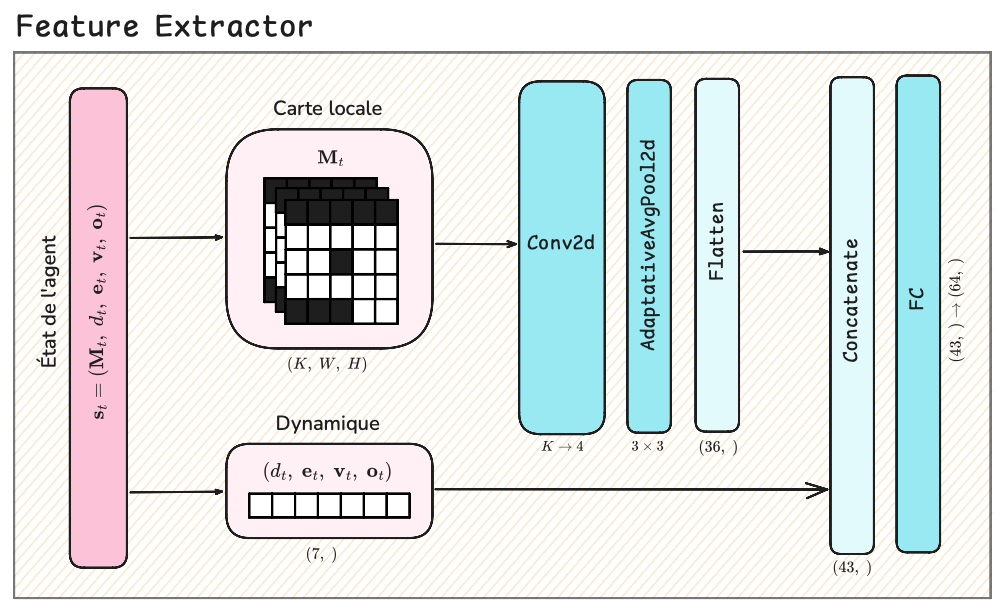
\includegraphics[scale=0.35]{figures/feature_extractor.png}
\end{figure}

\noindent L'ensemble des informations est ensuite projeté dans un espace latent de dimension fixe. Ce vecteur latent est fourni à un réseau entièrement connecté composé de deux couches cachées, illustré par la Figure \ref{fig:actor_network}. La sortie du réseau est divisée en deux branches : une première branche prédit la moyenne $\mu_\theta(\textbf{s})$ de la distribution d'action, tandis qu'une seconde branche prédit le logarithme de l'écart-type $\log \sigma_\theta(\textbf{s})$. Le logarithme de l'écart-type est borné afin d'éviter des valeurs trop grandes ou trop faibles, ce qui stabilise l'apprentissage.

\begin{figure}[h]
    \centering
    \caption{Architecture générale de l'actor network}
    \label{fig:actor_network}
    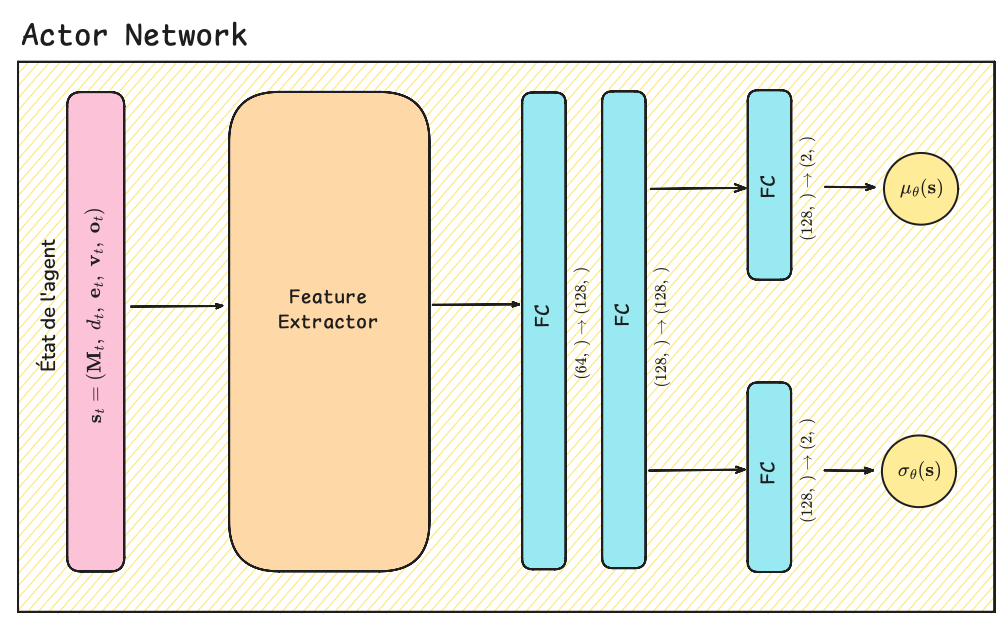
\includegraphics[scale=0.35]{figures/actor_network.png}
\end{figure}

\noindent À partir de ces deux sorties, une action est échantillonnée selon une loi gaussienne à l'aide du reparameterization trick. L'action est ensuite transformée par une fonction tangente hyperbolique, puis remise à l'échelle afin de respecter les bornes de l'espace d'action. L'action finale correspond donc aux deux commandes du robot : la vitesse linéaire $v_t$ et la vitesse angulaire $\omega_t$.

\vspace{10pt}

\noindent En phase d'évaluation, l'action n'est plus échantillonnée aléatoirement : on utilise directement la moyenne de la distribution, ce qui rend la politique déterministe et permet d'obtenir un comportement plus stable.


%%%%%%%%%%%%%%%%%%%%%%%%%%%%%%%%%%%%%%%%%%%%%%%%%%%%%%%%%%%%%%%%%%%%%%%%%%%%%%%%%%%%%%%

\subsubsection{Architecture des critic networks}

\noindent SAC utilise deux critic networks indépendants, notés $Q_{\phi_1}$ et $Q_{\phi_2}$. Ces deux réseaux ont la même architecture, illustrée par la Figure \ref{fig:critic_network}, mais leurs paramètres sont appris séparément. \textbf{Leur rôle est d'estimer la valeur d'une action donnée dans un état donné, c'est à dire $Q_\phi(\textbf{s}, \; \textbf{a})$.}

\vspace{10pt}

\noindent Comme pour l'actor, chaque critic commence par extraire une représentation latente de l'état. La carte locale est traitée par le même type d'extracteur convolutionnel, puis les caractéristiques obtenues sont concaténées avec les autres composantes de l'observation : distance à la cible, erreur d'orientation, vitesses et orientation du robot.

\vspace{10pt}

\noindent La différence principale avec l'actor est que le critic reçoit également l'action en entrée. Une fois le vecteur latent de l'état obtenu, celui ci est concaténé avec l'action $(v_t, \; \omega_t)$. Le vecteur résultant est ensuite traité par un réseau entièrement connecté composé de deux couches cachées. Cette dernière couche produit une valeur scalaire qui correspond à l'estimation de $Q_\phi(\textbf{s}, \; \textbf{a})$.

\begin{figure}[h]
    \centering
    \caption{Architecture générale des critic networks}
    \label{fig:critic_network}
    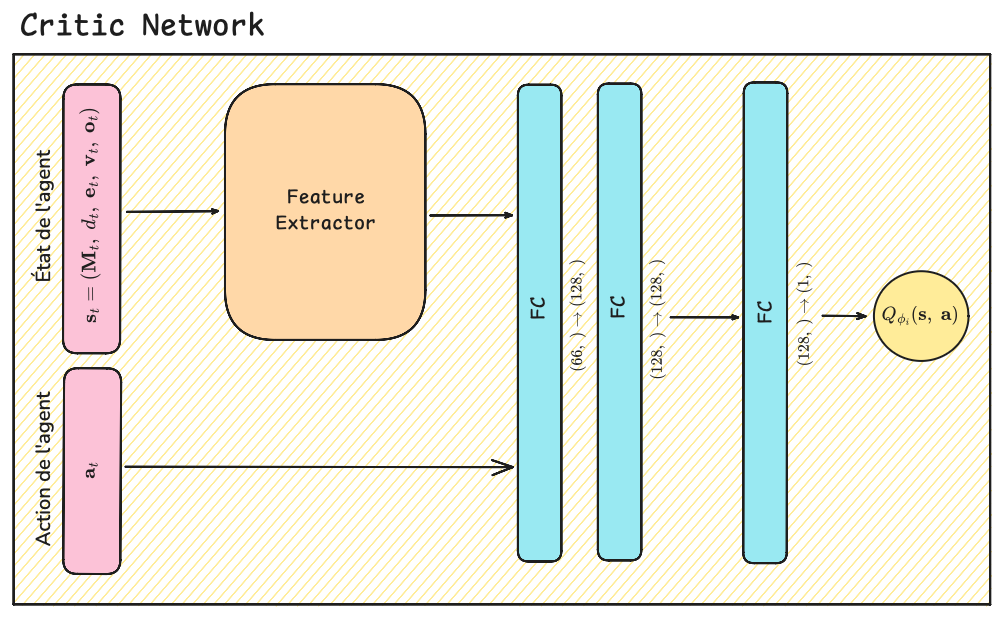
\includegraphics[scale=0.35]{figures/critic_network.png}
\end{figure}

\noindent L'utilisation de deux critic networks permet de limiter le biais de surestimation des valeurs $Q$. Lors du calcul des cibles d'apprentissage et de la mise à jour de l'actor, SAC utilise la plus petite des deux estimations, ce qui rend l'apprentissage plus stable.


%%%%%%%%%%%%%%%%%%%%%%%%%%%%%%%%%%%%%%%%%%%%%%%%%%%%%%%%%%%%%%%%%%%%%%%%%%%%%%%%%%%%%%%

\subsubsection{Normalisation des observations}

\noindent Les différentes composantes de l'état présentent des échelles de valeurs hétérogènes. Afin de faciliter l'apprentissage et d'éviter qu'une variable domine les autres, les observations sont normalisées avant d'être fournies aux réseaux de neurones.

\vspace{10pt}

\begin{itemize}
    \item La distance à la cible est normalisée par la diagonale de l'environnement afin d'obtenir une valeur comprise entre 0 et 1.

    \item Les vitesses linéaire et angulaire sont normalisées par leurs valeurs maximales autorisées.

    \item Enfin, les variables angulaires (orientation du robot et erreur d'orientation par rapport à la cible) sont représentées par leurs composantes trigonométriques $(\cos (\theta), \; \sin (\theta))$, ce qui permet d'éviter les discontinuités liées à une représentation angulaire directe.

    \item Les cartes locales étant binaires, elles ne nécessitent pas de normalisation supplémentaire.
\end{itemize}
